% !TEX root = ../report.tex

\chapter{Preliminary Study}
\minitoc

\clearpage

\section{State Of The Art}
\subsection{System Coldstart Handling}

Cold-start scenarios in recommender systems are situations in which little/no prior events, like ratings or clicks, are known for certain users or items. The cold start problem can divided into three sub problems: (1) Cold-start system, (2) Cold-start user and (3) Cold-start item

\subsubsection{Cold-start System}

%Having a large amount of data like e.g. in the netflix dataset
% -> Do not require a great understanding of the data to get decent results
% -> Out case is a little different. What implications does the limited amount of data have?

However, one situation when CF algorithms are less effective is when data is sparse, either because the target user is new to the system, an item is new, or both. In fact, in extreme cases, when data is very scarce, simple non-personalized recommendations based on global averages can outperform CF algorithms.

Most standard recommendation algorithms only word effectively in environments with datasets of high information density.

One difficult, though common problem for recommender systems is the cold-start problem.

Pure collaborative filtering cannot help in a cold-start setting, since no user preference information is available to form any basis for recommendations. However content information can help bridge the gap from existing items to new items, by inferring similarities among them.

%Approaches:
%Naive Filterbots - Covers (Cold start system, user & item)
%http://delivery.acm.org/10.1145/1160000/1150490/p699-park.pdf?ip=129.241.103.83&id=1150490&acc=ACTIVE%20SERVICE&key=CDADA77FFDD8BE08%2E5386D6A7D247483C2E4D4702B0C3E38B35%2E4D4702B0C3E38B35&CFID=419807217&CFTOKEN=62708098&__acm__=1394538962_5e2abb38bbcf4611b8354c8dd6abe53e

%Trust-Aware Collaborative Filtering for Recommender Systems
%http://download.springer.com/static/pdf/980/chp%253A10.1007%252F978-3-540-30468-5_31.pdf?auth66=1394714615_aa7f78fc8c1ed07f19406c3e36ff506f&ext=.pdf
% + Other articles as well


\subsubsection{Cold-start user}

\begin{quotation}
Ask the right questions if you're going to find the right answers
\end{quotation}
- Vanessa Redgrave

%What is the cold-start user problem?
Scenario: The target user has very few ratings (e.g. a new user). In this scenario, collaborative filtering (CF) based recommenders might not be able to find users with tastes that are truly similar to the target user, thus the recommendation quality to the target user might be poor. On the other hand, because of the very limited number of items rated by the target user, it is hard to obtain the content interests of the target user. Consequently, content-based techniques might only generate very limited recommendations in such situations.

One crucial problem of recommender system is how to best learn from new users. Collaborative Filtering (CF), is the best known technology for recommender systems and is based on the idea that like-minded users have similar tastes and preferences. A new user therefore poses a challenge to CF recommender, since the system has no knowledge about the preferences of the new user, and can therefore not provide any personalized recommendations, this is known as the cold start problem for new users. The system must therefore acquire some information about the new user in order to make personalized recommendations.

However, the system must be careful to present useful items to garner information. A food recommender should probably not ask whether a new user likes vanilla ice cream since most people like vanilla ice cream. Therefore, knowing that a new user likes vanilla ice cream tells you very little about the user. The choice of what questions to ask a new user, then, is critical.

Rashid et. al. \cite{Rashid2002} performed a study of different item selection strategies that collaborative filtering recommender systems can use to learn about new users. They presented the users with a questionnaire with items asking them to rate/select the ones they like. Their strategies can be divided into five classes:

\begin{itemize}
\item \emph{Random} strategies: Strategies that avoid bias in the presentation of bias
\item \emph{Popularity:} Select among the top N items where the probability that is proportionate to the items popularity.
\item \emph{Pure entropy:} Present the items with the highest entropy that the user has not seen
\item \emph{Balanced strategies:} A balanced approach combining both popularity data and entropy.
\item \emph{Personalized:} As soon as some information is known about a user, present items specifically tailored to that user using e.g. item-item similarity
\end{itemize}

This study was later extended by Rashid et. al. \cite{Rashid2008} where they more closely examined information theoretic strategies for item selection.

%Their suggestion for e-commerce: Recommend most popular items rather than the highest rated ones, and then use item-item similarity as quickly as possible

A new user preference elicitation strategy needs to ensure that the user does not 1) lose interest in returning due to low quality initial recommendations, 2) as quickly as possible being able to provide good personalized recommendations (find the right neighborhoods).

We are constrained to unobtrusively learn user-profiles from the natural interactions of users with the system, meaning that we can not require the user to rate e.g. 10 items before we can start providing recommendations. We have a \emph{mixed initiative} system meaning that there is provisions for both user and system controlled interactions. We (the system) can only select which items to recommend to the user, and this does not mean that the user actually will click an item or rate it.

%Addressing Cold-Start Problem in Recommendation Systems
%Hybrid approach - Analysis of two probabilsitic aspect models (pure collaborative filtering) to combine to users information
%http://delivery.acm.org/10.1145/1360000/1352837/p208-lam.pdf?ip=129.241.103.83&id=1352837&acc=ACTIVE%20SERVICE&key=CDADA77FFDD8BE08%2E5386D6A7D247483C%2E4D4702B0C3E38B35%2E4D4702B0C3E38B35&CFID=419807217&CFTOKEN=62708098&__acm__=1394540844_3a505da9cccf443d08f702408693d1f7

\subsubsection{Cold-start item}

%What is the cold-start item problem? / Introduction


%What strategies exist?


%What is suitable in our case?

\subsection{Fashion Recommendation}

% Building Recommender Systems using a Knowledge Base of product semantics
% http://images.accenture.ca/SiteCollectionDocuments/PDF/recommenderws02.pdf
% 	- Would probably require some more product semantics

%What are the challanges of making recommendations for fashion?
%	- How often are items relevant?
%	- Implicit feedback (Based around users fashion browsing habits and an occational purchase...)
%	- Changing interest of users
%	- Unstructured content/multiple content providers
%	- Sparsity
%	- Trends?

\subsection{Session Based Recommendation}
Init Hypothesis:
Two users with similar session habits and similar product accessing pattern have a stronger correlation to one-another than two users with just similar product interests.


'product\_purchase\_intended' (user pushed to the product web store) shows a wider specter of information about the product, including additional colors, images and colors.
For some it might be natural to explore the item there before "wanting" it. Making both

"product\_purchase\_intended" $\Rightarrow$ "product\_wanted"

and

"product\_purchase\_intended" $\notimplies$ "product\_wanted"

produce valuable information.

Must make different rules for the different stores:
"Bik Bok", "Cubus", "Gina Trik", "H\&M", "Bianco" has a broad specter of extra functions inside the web store, whereas others might not, only shows the product and a add to chart button.
This might divide the use pattern of the users into a:

"product\_detail\_clicked" $\Rightarrow$ "product\_purchase\_intended" $\Rightarrow$ "product\_wanted"

"product\_detail\_clicked" $\Rightarrow$ "product\_purchase\_intended" $\notimplies$ "product\_wanted",

and

"product\_detail\_clicked" $\Rightarrow$ "product\_wanted"

based on the store accessed.

Use this to make a "rule set" with a probability.
Then again use this to recommend items for the users with that given probability.

Find a "most popular session"-pattern
Find a "most likely to come after"-pattern

% db.sessions.group({key:{'storefront_name':1},cond:{},reduce:function(cur,result){result.count += 1}, initial: {count:0}})

Articles 4 l8er:
%http://dl.acm.org/citation.cfm?id=1136004
%http://link.springer.com/chapter/10.1007/3-540-46119-1_42
%http://dl.acm.org/citation.cfm?id=1082567
%http://link.springer.com/chapter/10.1007%2F978-3-540-30214-8_20
%http://dl.acm.org/citation.cfm?id=502935
%http://dl.acm.org/citation.cfm?id=1835896
%http://dl.acm.org/citation.cfm?id=345169
%http://dl.acm.org/citation.cfm?id=345169

Session issues:
Once in a blue moon a user will do a "product action" (purchase,want,details) without having a previous frontstore-access event. Which leads to unknown store-id of the item.
Issue is most probably from missing user-id in collection\_viewed, and a user checks out an item from there. It is not possible to be 100\% sure which user access the item from the collection\_viewed event, so this event is therefor not integrated into the session-stack.


% thoughts:
Categorize stores
    prize
    items in store

Categorize items
    Type
    Prize
    View frequency

Predicting events...
    Value brought vs. clustering on the "item"-events value

Make a store

% event_id, events:

% Products:
%     "product_detail_clicked",
%     "product_wanted",
%     "wantlist_menu_entry_clicked"
%     "product_purchase_intended",

% Store clicked: (produces not NULL storefront_name) (db.sessions.find({'storefront_name':{$ne:'NULL'},$or:[{'event_id':'featured_storefront_clicked'},{event_id:'storefront_clicked'}]}).count())
%     "storefront_clicked",
%     "featured_storefront_clicked",

% Other store interactions
%     "store_clicked",
%     "around_me_clicked",
%     "stores_map_clicked",
%     "collection_viewed",
%     "featured_collection_clicked",

% Start:
%     "app_first_started",
%     "app_became_active",
%     "app_started",
%     "user_logged_in",
%     "facebook_login_failed",

% Other:
%     "friend_invited",
%     "activity_clicked",
%     "facebook_share_changed",

% Course:
%     App started
%     Check next events, a days timeframe


%Simple session form, no structure:
% {u'event_id': u'product_detail_clicked', u'count': 68.0}
% {u'event_id': u'product_wanted', u'count': 35.0}
% {u'event_id': u'storefront_clicked', u'count': 69.0}
% {u'event_id': u'app_started', u'count': 26.0}
% {u'event_id': u'featured_storefront_clicked', u'count': 4.0}
% {u'event_id': u'user_logged_in', u'count': 9.0}
% {u'event_id': u'product_purchase_intended', u'count': 2.0}
% {u'event_id': u'around_me_clicked', u'count': 7.0}
% {u'event_id': u'stores_map_clicked', u'count': 1.0}
% {u'event_id': u'store_clicked', u'count': 1.0}
% {'user_id': 100001385800886L}
% {'num_events': 222}
% Total amount:    222
% User:            100001385800886
% Total Sessions:  30
% Total Events:    936
% Date:            11 - 10 - 2013

% Structured session exploration: Probably more info in this
% > db.sessions.find({'user_id':1094505588,session:64},{'event_id':1,'server_time_stamp':1,'_id':0}).sort({'ts':1})

% > db.sessions.find({'user_id':100000140823565,session:440},{'event_id':1,'server_time_stamp':1,'_id':0}).sort({'ts':1})

% > db.sessions.find({'user_id':100000140823565,session:440},{'product_id':1,'event_id':1,'_id':0}).sort({'ts':1})



\subsection{Recommenders (Similar systems? somethingsomething)}
\subsection{Items clustering}

% Trust based CF recommenders

% ### Hybrid Systems ###

% ### COLD START NEW ITEM ARTICLES ###

% Regression-based Latent Factor Models - http://dl.acm.org/citation.cfm?id=1557029
% Learning Attribute-to-Feature Mappings for Cold-Start Recommendations - http://ieeexplore.ieee.org/xpl/abstractCitations.jsp?tp=&arnumber=5693971&url=http%3A%2F%2Fieeexplore.ieee.org%2Fxpls%2Fabs_all.jsp%3Farnumber%3D5693971
% fLDA: Matrix Factorization through Latent Dirichlet Allocation - http://dl.acm.org/citation.cfm?id=1718499
% Matchbox: Large Scale Bayesian Recommendations


\section{Data Findings}
\subsection{What Can Be Understood From The Data}

%Dataset summary
	%How many users?
	%How much preference data?
	%Which events are interesting to look at?


\subsubsection{The Expected}
Event "app\_started", all have user\_id's
Event "app\_first\_started", all user\_id's are NULL
Event "user\_logged\_in", all have user\_id's... (assigned with login, event saved after login?)

\subsubsection{The Strange}
NULL valued  for user\_id events: (Not all strange, but put together for readability)
facebook\_share\_changed

collection\_viewed  ignoring collection view-event as of now since the user\_id is null. Could be valuable to use, though (30 000 events ignored) ...
potential workaround:
    for each session do:
        Filter all events on:
            session-ts-start to session-ts-end,
            allow: user\_id session-user-id and NULL
            Ip of user-session and ip of collection\_viewed
            storefront\_id's from session
                Populate collection\_viewed-user-id with session-user-id
Potential faulty user-id setting for ip-switch during a session, but expect few occurrences of this

wantlist\_menu\_entry\_clicked
app\_became\_active

app\_first\_started
facebook\_login\_failed

> db.prod.distinct('event\_json.ipAddress').length
9033
> db.prod.distinct('event\_json.eventData.device\_id').length
2644
> db.prod.distinct('user\_id').length
1660

More devices than users, can't fill the blanks with device\_id

Q's:
    app\_became\_active id's for better sessions?
    store\_clicked vs. storefront\_clicked (23 vs. 19744)
    API item-id's mapping to event product\_id's; how to map?



soBazar want to build a proper model.
Give input on how to build this model. The supplier should know that an item is a jacket for instance.
Have something to show on the 20. Should be better than what is already implemented.



\subsection{Graphs}

Interesting fields from data:

    Events: userid - prodid - storeid - time - price? - applicationstate - (eventlocation)

    Offer: prodid - price(old/new) - storeid -time -

Thoughts on graphs (some of these will be in the appendix/removed, placed here for simplicity and structure) (event database filtered on "server-environment" with "prod" as value and removed all events with "simulator" as "platform"):



    Simple:

\begin{table}
    \begin{tabular}{l|l|l}
    ~                                                 & Amount                                                                                                                                                                                            & Notes                                                                                                                                                                                                                \\ \hline
    Unique users                                      & 1658                                                                                                                                                                                              & Count of unique users in eventdatabase                                                                                                                                                                               \\ \hline
    > db.prod.distinct('product\_name').length & 2591                                                                                                                                                                                              & Count for unique items                                                                                                                                                                                               \\ \hline
    > db.prod.distinct('product\_id').length & 4042                                                                                                                                                                                              & Count for unique items                                                                                                                                                                                               \\ \hline
    > db.offer.distinct('brandId').length             & 15                                                                                                                                                                                                & Count stores unique (not collections, but from offer\\(the items database) db)  (The missing 4 (the last two\\are null and N/A). These are foreign brands i.e. unknown,\\maybe test brands. 45002,38002,44004,55006) \\ \hline
    > db.prod.distinct('retailer\_brand').length & 21                                                                                                                                                                                                & Count stores unique (from prod db)                                                                                                                                                                                   \\ \hline
    Items in events not in the actual offer database: &         NonMatching values:             620\\        Offer database length:          7854\\        Event items length:             4042\\        Items from list2 not in list1:  7.89406671759613 & ~                                                                                                                                                                                                                    \\ \hline
    ~                                                 & ~                                                                                                                                                                                                 & ~                                                                                                                                                                                                                    \\ \hline
    ~                                                 & ~                                                                                                                                                                                                 & ~                                                                                                                                                                                                                    \\ \hline
    ~                                                 & ~                                                                                                                                                                                                 & ~                                                                                                                                                                                                                    \\ \hline
    ~                                                 & ~                                                                                                                                                                                                 & ~                                                                                                                                                                                                                    \\ \hline
    ~                                                 & ~                                                                                                                                                                                                 & ~                                                                                                                                                                                                                    \\ \hline
    ~                                                 & ~                                                                                                                                                                                                 & ~                                                                                                                                                                                                                    \\ \hline
    ~                                                 & ~                                                                                                                                                                                                 & ~                                                                                                                                                                                                                    \\
    \end{tabular}
\end{table}

        Price ranges of all items (groupings)

\begin{figure}[H]
    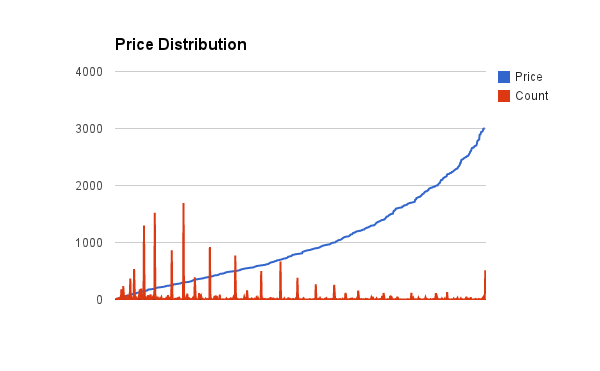
\includegraphics[width=5in]{image/price_distr.png}
    \centering
    \caption[Price distribution of items]{some awesome text}
    \label{figure:ratingdistr}
\end{figure}

        (Distinct event locations)TODO

        Item time on market TODO maybe not that interesting alone


    complex 2.Deg:

        Count for different events

\begin{figure}[H]
    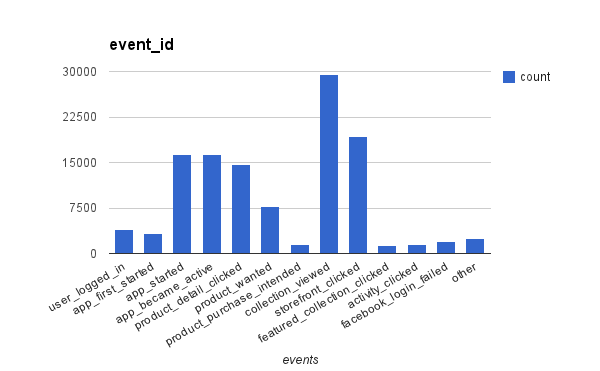
\includegraphics[width=5in]{image/event_id.png}
    \centering
    \caption[Count for different events]{some awesome text}
    \label{figure:ratingdistr}
\end{figure}

        Distinct events done on stores (shady)

\begin{figure}[H]
    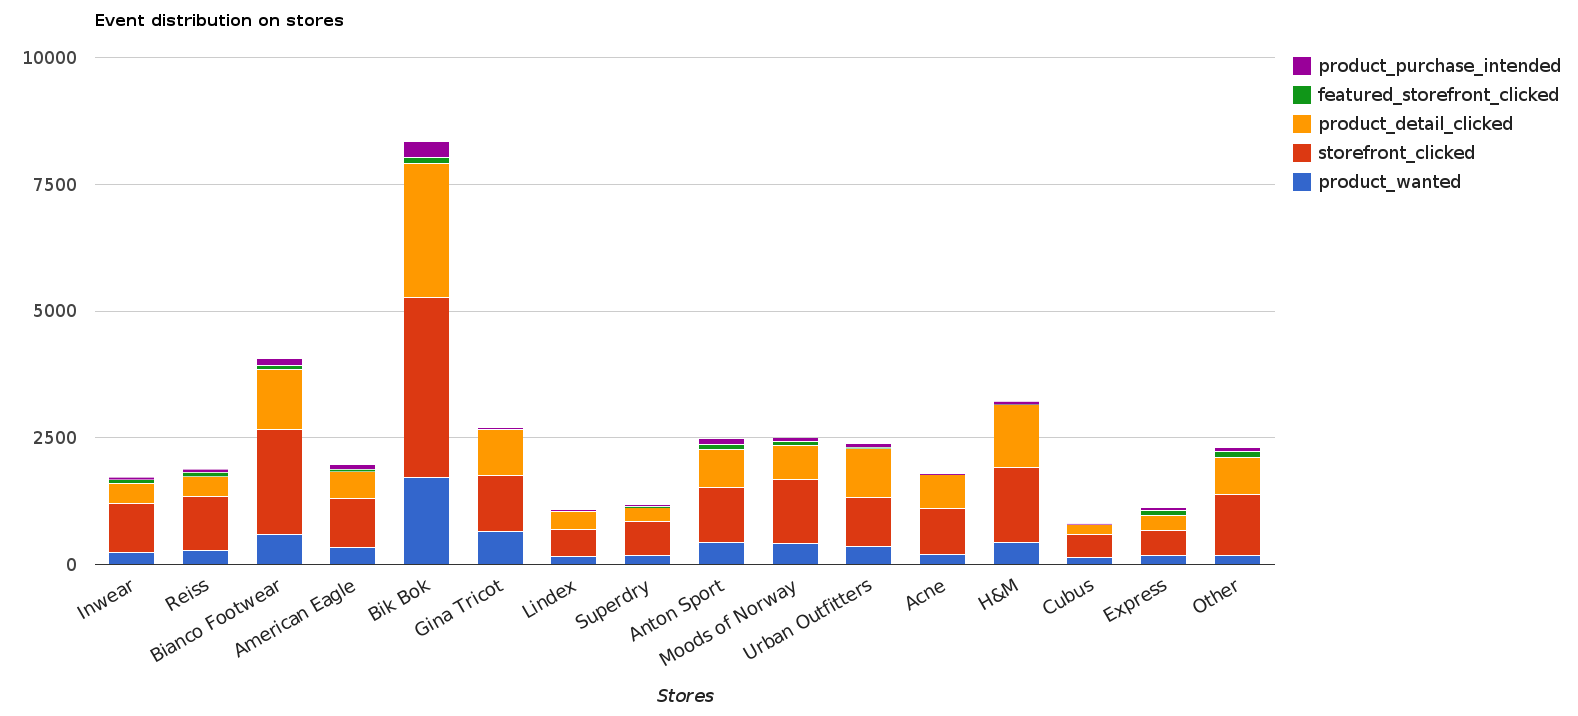
\includegraphics[width=5in]{image/event_distr.png}
    \centering
    \caption[Distribution of events on storefronts]{some awesome text}
    \label{figure:ratingdistr}
\end{figure}

\begin{figure}[H]
    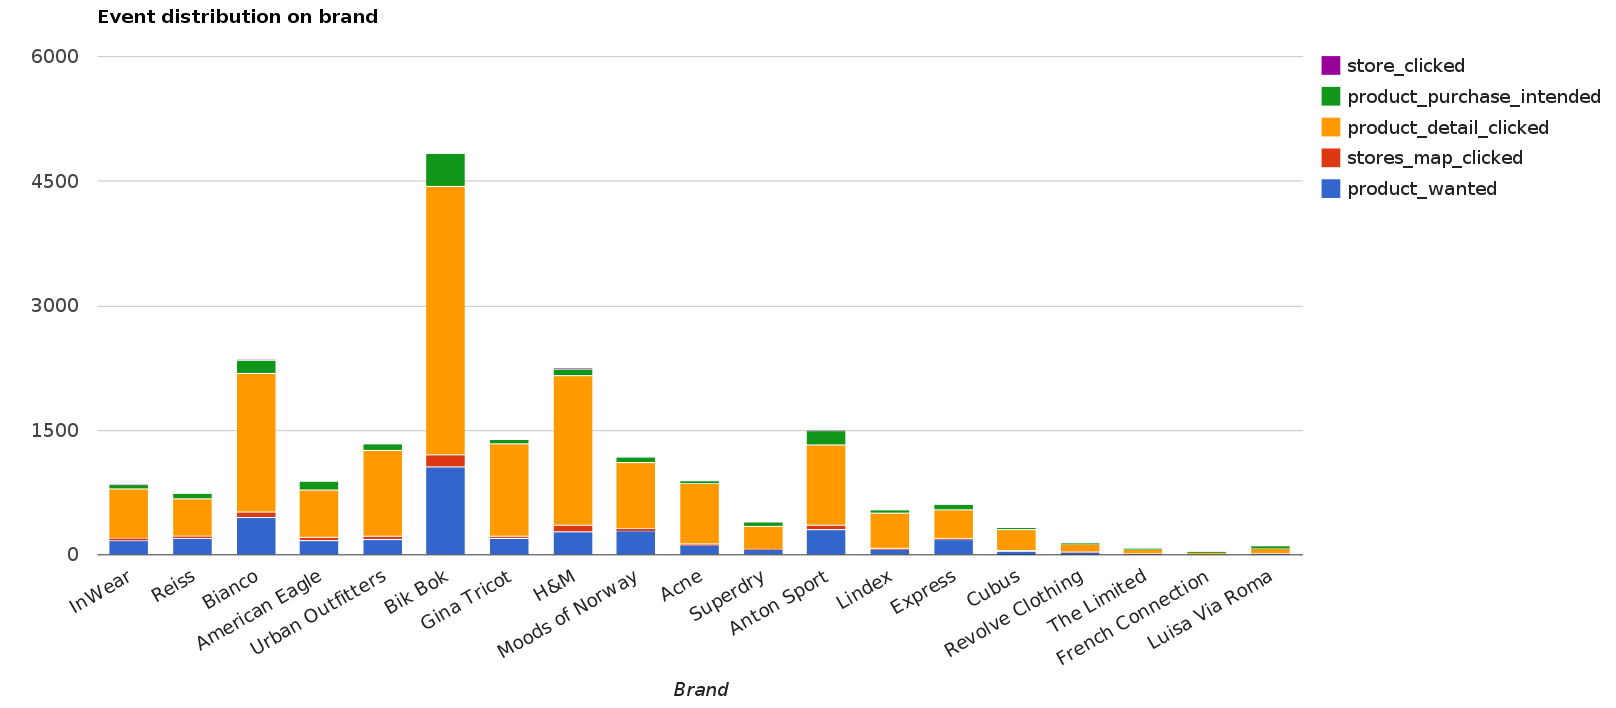
\includegraphics[width=5in]{image/brand_distr.png}
    \centering
    \caption[Distribution of events on brands]{some awesome text}
    \label{figure:ratingdistr}
\end{figure}

        peak online (slope-style) (events per day)

\begin{figure}[H]
    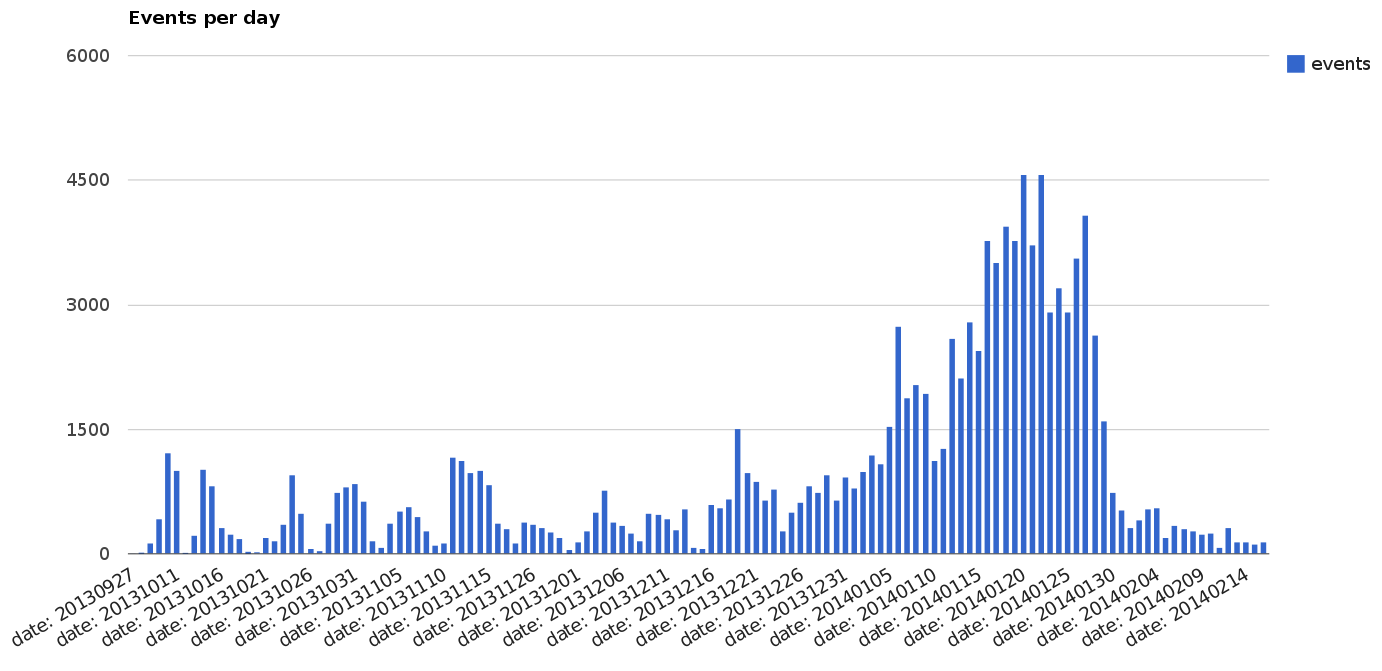
\includegraphics[width=5in]{image/events_per_day.png}
    \centering
    \caption[Distribution of events per day]{TODOsome awesome text}
    \label{figure:ratingdistr}
\end{figure}


        Price range of items in stores
        count User eventes
        user-item (how many items has a user "interacted" with)
        Count of unique items in item db also in event db
        Usable events regarding userid (events types with not null userid)
        (Plotting locations)
        unique Stores count for users

    complex 3.Deg:

        count Sessions for users (aprox: sessioncount)TODO

\begin{figure}[H]
    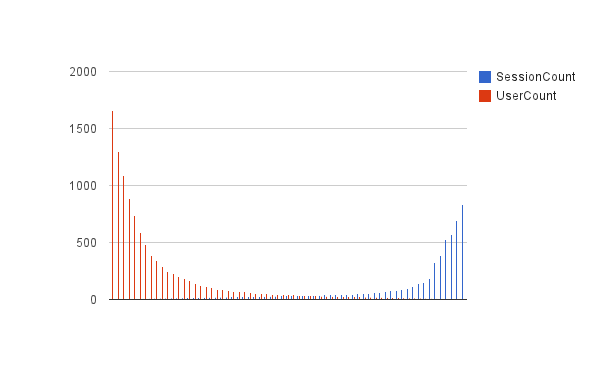
\includegraphics[width=5in]{image/global_sessioncount.png}
    \centering
    \caption[Count of sessions per user mapped with count of user with give session amount]{TODOsome awesome text}
    \label{figure:ratingdistr}
\end{figure}

        price span for user

    complex 4.Deg:

        Stats for sessions:

            Timespann of sessions for users (avg, max, min)
            Events per session (avg, max, min)
            Item viewtime for user in session
            Stores visited per session
            revisit time of items for user
            relationship with view, want and purchase
            time of session over lifetime of app
            user preferred price in session

    complex 5.Deg:

        Stats for global session stats:

            price vs view, want and purchase
            avg viewtime for an item (i know)
            Similarity of user favorite store, items viewed and items wanted?
            time of session over lifetime of app for all users (slope-style)

    complex 6.Deg:

TODO: STRUCTURExfdgdsagCFG
SDFG

    Blobs of smaller bubbles with eventid
    Blobs for eventcount on stores with items items from stores (populate "storename" for "itemevents")
    Show occurence of event after other event?
    User stats: items, likes, intented purchased, events, session avg, max event, fequency
    Find prices for stores: prize ranges
    User

Visuals:
    BubbleChart

To be done to 17:
    - PP
    - List articles to be read
    - Prototype implementation
    - Research question(s)
    -


\section{What to use}


%
\subsection{Some Awesome Algorithms (Build up with project progress)}

Given enough data, item-based CF methods often performs as well or better than almost any other recommendation method. However, in cold-start situations where a user, an item, or the entire system is new, simple non-personalized recommendations often fare better...

User based - new user
Non personalized approaches
	- most popular
	- highest rated
Other alternatives
	- use demographic information

Item based - new item
	- most popular
	- highest rated
	- use content information

When you enter a clothing store you are normally confronted with the following suggestions:
	- New in/Seasonal highlights
	- Special offer/discounts
	- Bestsellers
	- Are you looking for something in particular?

Personalized recommendations, what assumptions can be made?
\#1 - You are like your friends
\#2 - You are like people who do similar things that you do
\#3 - You like things that are similar to things you already like
\#4 - You are influenced by experts and the opinions of others

\subsubsection{The Good}
\subsubsection{The Bad}
\subsection{Why Not To Use These (Same As above)}
\subsubsection{The Good}
\subsubsection{The Bad}

\section{How to evaluate}


Some key questions in evaluating recommender systems on testbed data are: what to predict, how to grade performance and what baseline to compare with.


Explicit feedback ("relevance judgement")

Explicit feedback are more precise than implicit feedback, but more difficult to collect since it requires the user to spend time rating items and the amount of feedback is often scarce. The main difference between the two is that implicit feedback is inferred from user behaviour, such as noting which news articles they do and do not view. Explicit feedback unlike implicit feedback provides the users with a mechanism to unequivocally express their ratings on a scale from usually in the form of a Likert scale ranging from 1-5 (strongly disagree - strongly agree). Thus explicit feedback captures both positive and negative feedback, while implicit feedback only can be positive. Furthermore, explicit feedback tend to concentrate on either side of the rating scale, as users are more likely to express their preference if they feel strongly for or against an item.

product\_wanted, in the form of like/no feedback, can this be considered "explicit feedback?" no negative feedback...

Implicit feedback (Indirectly reflect opinion through observing user behaviour)

Unlike the more extensively researched explicit feedback, we do not have any
direct input from the user regarding their personal preferences. In particular
we do not have any substantial evidence of which items the user dislikes (e.g. a
low rating for a movie). But in return implicit feedback is more easily
collected, and usually more abundant.

Almost all of the research on implicit feedback has considered how behaviors can
be used as positive evidence, rather than negative evidence. However, one can imagine
behaviors which indicate that a user does not find something relevant or which suggest
that something is unimportant to the user, such as delete. It is likely that little research
has been conducted on negative implicit feedback because there are fewer of these types
of behaviors, and, in general, less is understood about how to effectively use negative
feedback, whether for implicit or explicit relevance feedback.

Another challenge facing implicit feedback research is the notion of degree of
personalization offered by the system. In particular, individual differences can greatly
impact the effectiveness of using behavior as implicit relevance feedback. People behave
differently and have varying approaches to information-seeking; thus, it is difficult to
generate, and dangerous to apply, all-purpose rules for describing how behavior can be
used as implicit relevance feedback

%Implicit feedback classfication (Type, confidence, precision)

In the case of our project we collect the following data, which can be considered as implicit feedback.
- product\_detail\_clicked, product\_purchase\_intended, collection\_viewed(?)...

Other types of implicit feedback include purchase history, browsing
history, search pattern and even mouse movements

Hu et. al. \cite{Hu2008} identify four unique characteristics of implicit feedback, which differentiates it from explicit feedback...

\begin{enumerate}

\item No negative feedback. By observing user behaviour we can infer which items the user consume and probably like. However, it is hard to infer
which items the user did not like. This asymmetry has several implications; Explicit feedback provides a more detailed picture of the
users preferences, but for implicit data the low ratings are treated as missing data and omitted from the analysis. Hence it is crucial to address
the missing data where most negative feedback is expected to be found

\item Implicit feedback is inherently noisy. While we track user behaviour, we can only guess their preferences and true motives. For example, a
purchase does not necessarily indicate a positive view of an item, the item may have been purchased as a gift, or perhaps the user was disappointed
with the item

\item The numerical value of explicit feedback indicates preference, whereas the numerical value of implicit feedback indicates confidence. Explicit
feedback could e.g. range from total dislike to really like, on the other hand implicit feedback describe the frequency of actions, e.g. how
frequently a user buys an item. But a higher frequency might not necessarily indicate a stronger preference. A user might choose to only
watch a really good movie once. However, a recurring event is more likely to reflect the user opinion. However, the numerical value of the feedback
is definitely useful, as it tells us about the confidence we have in a certain observation

\item Evaluation of implicit feedback requires appropriate measures. In the case of explicit feedback where a user specify a numerical score, measures such
as mean squared error (MSE) could measure the success of the predictions. However, with implicit models we have to take into account
the availability of the item, competition with other items, and repeat
feedback.

\end{enumerate}

Accuracy metrics not suited for implicit feedback datasets, as they require knowing which items are undesired by a user \cite{Hu2008}.

Being accurate is not always enough. Striking a balance between accuracy and user satisfaction \cite{McNee2006}
	% High accuracy != User satisfaction
	% Therefore, important to consider other evaluation metrics beyond the conventional ones
	% Which are the most important factors to consider with regards to user satisfaction

The data available strongly influences the choice of evaluation method/metrics. E.g. classification accuracy metrics seem to be the most suitable when working with binary preferences, e.g. in the form of recall-oriented measures.

\subsection{What Has Been Done Before}

%Evaluation by looking at sessions
%Evaluation using implicit feedback datasets
%Turnover rate?
% ++

%Clues
% http://delivery.acm.org/10.1145/570000/564421/p253-schein.pdf?ip=129.241.103.83&id=564421&acc=ACTIVE%20SERVICE&key=CDADA77FFDD8BE08%2E5386D6A7D247483C%2E4D4702B0C3E38B35%2E4D4702B0C3E38B35&CFID=419807217&CFTOKEN=62708098&__acm__=1394537427_86c608d0d7733db023faa5a09da46de7

\subsection{What To Use}
\subsubsection{The Good}
\subsubsection{The Bad}

\section{Evaluation}



Thoughts:

